\documentclass[crop,tikz]{standalone}
\usepackage{amsmath}
\usepackage{amsfonts}
\usepackage{physics}
\usepackage{tikz}
\usetikzlibrary{shapes}
\usepackage{dsfont}
\usepackage{bbm}
% parameters for the MPS drawings
\definecolor{Tcolor}{RGB}{255, 235, 171}
\definecolor{Wcolor}{RGB}{190, 190, 255}
\def\textoffsetVertical{0.8}
\def\nodewidth{0.6*28.5}
\def\legwidth{0.8}
\def\nodedistance{1.25}
\def\textoffsetVerticalW{0.9}
\def\textoffsetHorizontalW{-0.9}
\def\textoffsetVerticalMPO{1.2}
\def\yoffset{1}
\def\xoffset{3}
\def\resultMPSYoffset{2.5}
\def\resultMPSXOffsetSmall{2}
\def\resultMPSXOffset{3}
\def\dotsOffset{3}
\def\conjOffsetVertical{1.25}
\def\conjOffsetVerticalLarge{2.2}
\def\curvedLineXOffset{0.7}
\def\cmscale{28.5}
\def\miniatureScale{0.5}
\def\Heffheight{1.2*28.5}
\def\Heffwidth{4.0*28.5}
\def\Heffonewidth{3.0*28.5}
\def\miniatureTextOffsetVertical{0.5}
\begin{document}
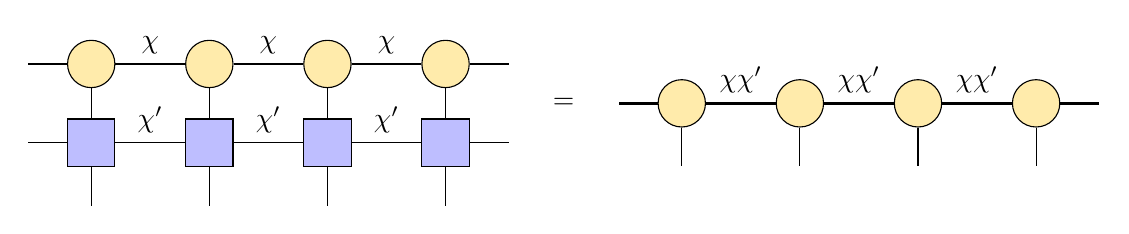
\begin{tikzpicture}[baseline=(current  bounding  box.center)]
    \def\nodedistancemultiplier{1.2}
    % MPS
    \node[draw, shape=circle, fill=Tcolor, minimum width=\nodewidth] (T1) at (0, 0) {};
    \node[draw, shape=circle, fill=Tcolor, minimum width=\nodewidth] (T2) at ({1*\nodedistance*\nodedistancemultiplier}, 0) {};
    \node[draw, shape=circle, fill=Tcolor, minimum width=\nodewidth] (T3) at ({2*\nodedistance*\nodedistancemultiplier}, 0) {};
    \node[draw, shape=circle, fill=Tcolor, minimum width=\nodewidth] (T4) at ({3*\nodedistance*\nodedistancemultiplier}, 0) {};
    \draw (T1) -- node[midway,above] {$\chi$} (T2);
    \draw (T2) -- node[midway,above] {$\chi$} (T3);
    \draw (T3) -- node[midway,above] {$\chi$} (T4);
    \draw (T1) -- ++(-\legwidth, 0);
    \draw (T4) -- ++(\legwidth, 0);
    % MPO
    \node[draw, shape=rectangle, fill=Wcolor, minimum width=\nodewidth, minimum height=\nodewidth] (W1) at (0, -\yoffset) {};
    \node[draw, shape=rectangle, fill=Wcolor, minimum width=\nodewidth, minimum height=\nodewidth] (W2) at ({\nodedistance*\nodedistancemultiplier}, -\yoffset) {};
    \node[draw, shape=rectangle, fill=Wcolor, minimum width=\nodewidth, minimum height=\nodewidth] (W3) at ({2*\nodedistance*\nodedistancemultiplier}, -\yoffset) {};
    \node[draw, shape=rectangle, fill=Wcolor, minimum width=\nodewidth, minimum height=\nodewidth] (W4) at ({3*\nodedistance*\nodedistancemultiplier}, -\yoffset) {};
    \draw (T1) -- (W1);
    \draw (T2) -- (W2);
    \draw (T3) -- (W3);
    \draw (T4) -- (W4);
    \draw (W1) -- node[midway,above] {$\chi^\prime$} (W2);
    \draw (W2) -- node[midway,above] {$\chi^\prime$} (W3);
    \draw (W3) -- node[midway,above] {$\chi^\prime$} (W4) -- ++(\legwidth, 0);
    \draw (W1) -- ++(-\legwidth, 0);
    \draw (W1) -- ++(0, -\legwidth);
    \draw (W2) -- ++(0, -\legwidth);
    \draw (W3) -- ++(0, -\legwidth);
    \draw (W4) -- ++(0, -\legwidth);
    % equal sign
    \node[] (eq) at ({3*\nodedistance*\nodedistancemultiplier+\resultMPSXOffset/2}, -\yoffset/2)  {$=$};
    % result MPS
    \node[draw, shape=circle, fill=Tcolor, minimum width=\nodewidth] (Tp1) at ({3*\nodedistance*\nodedistancemultiplier+\resultMPSXOffset}, -\yoffset/2) {};
    \node[draw, shape=circle, fill=Tcolor, minimum width=\nodewidth] (Tp2) at ({4*\nodedistance*\nodedistancemultiplier+\resultMPSXOffset}, -\yoffset/2) {};
    \node[draw, shape=circle, fill=Tcolor, minimum width=\nodewidth] (Tp3) at ({5*\nodedistance*\nodedistancemultiplier+\resultMPSXOffset}, -\yoffset/2) {};
    \node[draw, shape=circle, fill=Tcolor, minimum width=\nodewidth] (Tp4) at ({6*\nodedistance*\nodedistancemultiplier+\resultMPSXOffset}, -\yoffset/2) {};
    \draw[very thick] (Tp1) -- node[midway,above] {$\chi\chi^\prime$} (Tp2);
    \draw[very thick] (Tp2) -- node[midway,above] {$\chi\chi^\prime$} (Tp3);
    \draw[very thick] (Tp3) -- node[midway,above] {$\chi\chi^\prime$} (Tp4);
    \draw[very thick] (Tp1) -- ++(-\legwidth, 0);
    \draw[very thick] (Tp4) -- ++(\legwidth, 0);
    \draw (Tp1) -- ++(0, -\legwidth);
    \draw (Tp2) -- ++(0, -\legwidth);
    \draw (Tp3) -- ++(0, -\legwidth);
    \draw (Tp4) -- ++(0, -\legwidth);
\end{tikzpicture}
\end{document}